\documentclass{article}

% NeurIPS 2026 style in preprint mode: no line numbers,
% authors shown. Keep neurips_2026.sty unmodified.
% Numeric citations, numbered in order of first citation.
\PassOptionsToPackage{numbers,sort&compress}{natbib}
\usepackage[preprint]{neurips_2026}

% Label the first-page footer as a technical report, not a preprint of a
% later paper. Overridden here so the style file stays unmodified.
\makeatletter
\renewcommand{\@noticestring}{Technical report.}
\makeatother

% Plain "Acknowledgments" heading instead of the style's
% "Acknowledgments and Disclosure of Funding".
\renewcommand{\acksection}{\section*{Acknowledgments}}

\usepackage[utf8]{inputenc}
\usepackage[T1]{fontenc}
\usepackage{hyperref}
\usepackage{url}
\usepackage{booktabs}
\usepackage{amsmath}
\usepackage{amsfonts}
\usepackage{amssymb}
\usepackage{nicefrac}
\usepackage{microtype}
\usepackage{xcolor}
\usepackage{graphicx}
\usepackage{subcaption}
\usepackage{multirow}
\usepackage{fvextra} % verbatim prompt listings with line breaks
\usepackage[capitalize,noabbrev]{cleveref}

\graphicspath{{assets/}}

\hypersetup{
    colorlinks=true,
    linkcolor=blue!50!black,
    citecolor=blue!50!black,
    urlcolor=blue!50!black
}

% Drafting markers; remove every use before upload (`make check` lists them).
\newcommand{\todo}[1]{\textcolor{red}{[TODO: #1]}}

% \endofdump marks where the precompiled preamble stops (mylatexformat).
% Define it as a no-op so normal builds, Overleaf and arXiv ignore it.
\ifdefined\endofdump\else\let\endofdump\relax\fi

\endofdump % the precompiled preamble stops here (see Makefile); a no-op otherwise

\title{Lightweight Restraints for Powerful Agents: AI Control Monitors That Decide in One Forward Pass}

\author{%
    Jeremias Ferrao\thanks{Corresponding author: \texttt{j.lino.ferrao@gmail.com}.} \\
    Safe AI Netherlands
    \And
    Abhinav Rajeev Kumar \\
    Independent
}

\hypersetup{
    pdftitle={Lightweight Restraints for Powerful Agents: AI Control Monitors That Decide in One Forward Pass},
    pdfauthor={Jeremias Ferrao and Abhinav Rajeev Kumar}
}

\begin{document}

\maketitle

\begin{abstract}
\todo{Abstract: problem (monitoring on the critical path of agent actions), method (binary-logit distillation from a frontier teacher into small open-weight monitors), headline results, and what is released, with one link to the project page that gathers the code, weights, teacher probabilities and serving image.}
\end{abstract}

\section{Introduction}
\label{sec:introduction}

\todo{Motivate cheap, fast monitors: the safety tax of frontier monitors on the critical path of agent actions.}

\todo{State contributions as a short list: training recipe, evaluation, analysis, released models and serving stack. The release bullet lists the code, adapters and merged checkpoints, teacher probabilities and serving image, the MIT licence and the project page; the conclusion only says what others can do with them.}

\section{Background and related work}
\label{sec:background}

\paragraph{Two uses of monitors.}
Monitors score the actions of an AI agent, and deployed systems use the scores in two ways.
The first use is to select actions for human audit.
In the trusted monitoring protocol of AI control~\citep{greenblatt2023ai}, a trusted model rates how suspicious each output of an untrusted model looks.
Humans audit the outputs with the highest ratings, as far as their time allows.
The second use is to decide whether an action may run.
In the auto mode of Claude Code~\citep{anthropic2026auto} and the auto-review of Codex~\citep{openai2026autoreview}, a separate model approves or blocks an action before it runs.
A blocked action returns to the agent with the reason, and a human is asked only after repeated blocks.
Both uses need a monitor that separates harmful from benign actions at a low false-positive rate.
A false positive spends audit time in the first use and interrupts the agent in the second.
In both uses the monitor runs on each action it covers, so its cost adds to every such action.
In the second use the action also waits for the monitor.

\todo{Sinha et al.~\citep{sinha2026training} in a quarter to half a page: training data and rationale pipeline, OOD suite, pAUROC@20, cost axis. State that these monitors are action-only: they read the visible trajectory, not the reasoning or activations of the agent. Close with what we reuse and what we change.}

\todo{Decision models from industry (model cards, no technical reports).}

\todo{Activation probes in production~\citep{kramar2026building,cunningham2026constitutional}; monitor-directed attacks~\citep{terekhov2025adaptive}.}

\section{Training and serving Gleipnir monitors}
\label{sec:method}

\subsection{Monitor input and output}
\label{sec:interface}

A Gleipnir monitor reads one trajectory and returns one score.
The input is a single user message: an instruction that describes harmful behavior, followed by the trajectory between \texttt{<agent\_trajectory>} tags.
Appendix~\ref{app:prompts} gives the instructions in full, and Appendix~\ref{app:data-discrepancies} describes what the trajectories contain.
We apply the chat template of the model with thinking disabled and start the reply of the model with the text \texttt{Prediction:}.
The monitor then reads the logits $z_0$ and $z_1$ of the tokens \texttt{0} (benign) and \texttt{1} (harmful) at the next position.
The score is the probability of \texttt{1} among these two tokens,
\begin{equation}
s = \frac{e^{z_1}}{e^{z_0} + e^{z_1}} = \sigma(z_1 - z_0) .
\label{eq:score}
\end{equation}
This output has two properties that the output of Section~\ref{sec:background-sinha} lacks.
It needs one forward pass over the prompt and no generated text, so the monitor writes no rationale.
It is also continuous, so it ranks trajectories without the ties of an integer scale.

\paragraph{Effect of the output format.}
The output format changes the score of a monitor before any training.
We compare four formats on the unadapted Qwen3.5-9B, with the model, the OOD suite and the monitoring specification fixed; only the wording of the output instruction differs.
Binary logits score 0.698 Mean-OOD.
An integer from 0 to 10 scores 0.486.
Rounding the binary scores to one decimal lowers Mean-OOD by only 0.014, so the coarser scale does not explain this difference.
When the model writes its reasoning before the output, the integer scores 0.666 and the binary logits score 0.692, in both cases at a higher cost (Table~\ref{tab:ood-all}).
Binary logits without reasoning are therefore the cheapest of the four formats and score at least as high as the others.

\subsection{Soft-target distillation}
\label{sec:binary-logit-distillation}

We train the monitor to match the probability that a stronger teacher model gives to the decision token.
The teacher is Kimi K3.
It reads each training trajectory with the full specification (Appendix~\ref{app:prompts}) and answers with one decision token, without reasoning.
We read the log-probabilities of \texttt{0} and \texttt{1} for this token and normalize them as in Equation~\ref{eq:score}, which gives the teacher probability $p$.
We compute $p$ once for each of the 8,688 training trajectories and store it.
The loss of the monitor on a trajectory is the binary cross-entropy between its score $s$ and the teacher probability,
\begin{equation}
\mathcal{L} = -\,p \log s - (1 - p) \log (1 - s) .
\label{eq:loss}
\end{equation}
The loss has no term for the source label and no temperature.
In contrast to the pipeline of Section~\ref{sec:background-sinha}, the teacher writes no rationale, and no judge model or RL stage is needed.

\paragraph{Teacher-agreement filter.}
We use the source labels only to filter the training set.
We remove a trajectory when the decision of the teacher ($p \geq 0.5$) disagrees with its source label, which removes 852 of the 8,688 trajectories and leaves 7,836.
In a comparison on one seed of the 4B, the filter raised pAUROC@20 on the validation set from 0.847 to 0.896.
It also raised the false-positive rate at a threshold of 0.5 from 5.3\% to 21.4\%, so the filter improves the ranking of the monitor but not its calibration at this threshold.
This comparison has no control that removes the same number of trajectories at random.

\paragraph{Soft targets against hard labels.}
We test the effect of the soft targets by training on the source labels instead, with all other settings unchanged.
For the 4B, we compare three seeds for each objective.
With hard labels the seeds score 0.690 to 0.746 Mean-OOD, and with soft targets they score 0.777 to 0.813; the means are 0.716 and 0.792, a difference of 0.076.
On the validation set the means are 0.833 and 0.903.
For the 27B, we have one seed for each objective, and the difference is smaller.
With the compact instruction and BF16 serving, hard labels score 0.904 Mean-OOD and soft targets score 0.909.
In the configuration that we release (Sections~\ref{sec:training-setup} and~\ref{sec:serving}), they score 0.933 and 0.951.
On the validation set, the hard-label 27B scores higher in that configuration, 0.959 against 0.944.
Its scores are also less graded: 80\% of its OOD scores lie within 0.01 of 0 or 1, against 20\% for the soft-target 27B.
Soft targets therefore help the 4B on both sets, and for the 27B they help the OOD score and the spread of the scores but not the validation score.
One explanation is that soft targets add less when the unadapted model is already close to the teacher.
We cannot separate this from the size of the model with two models, and we leave it open.

\subsection{Training setup}
\label{sec:training-setup}

\todo{Data, LoRA configuration, the two instructions, seed averaging for the 4B, the instruction choice for the 27B, quantization-aware distillation.}

\subsection{Serving and cost}
\label{sec:serving}

\todo{Main serving decisions: single prefill pass, low-precision weights with QAD for the 4B, last-token final-layer attention, host-path changes. Cost per 1,000 evaluations at on-demand and committed-use B200 rates. Score change against BF16 serving. Released artifacts. Throughput per change goes in the appendix.}

\section{Serving and cost}
\label{sec:serving}

\todo{Main serving decisions: single prefill pass, low-precision weights with QAD for the 4B, last-token final-layer attention, host-path changes. Cost per 1,000 evaluations at on-demand and committed-use B200 rates. Score change against BF16 serving. Released artifacts. Throughput per change goes in the appendix.}

\section{Main evaluation}
\label{sec:evaluation}

We compare monitors on the OOD suite of Sinha et al.\ (Section~\ref{sec:background}) by Mean-OOD pAUROC@20 and by the cost of 1,000 evaluations.
The reasoning monitors are those of Sinha et al., with the scores and costs that they report.
We scored decision models and unadapted language models ourselves, from their binary logits or native probabilities, and price them at API or hosted prices.
We price Gleipnir at the cost of one B200 with one request at a time, at both rates of Section~\ref{sec:serving}, on the released serving stack.
Gleipnir 4B reads the compact instruction and Gleipnir 27B the full specification (Section~\ref{sec:training-setup}).
Figure~\ref{fig:frontier} shows the main comparisons. Table~\ref{tab:ood-all} in Appendix~\ref{app:ood-all} lists every monitor, together with its recall at a false-positive rate of 1\%, which is closer to deployment.

\begin{figure}[t]
\centering
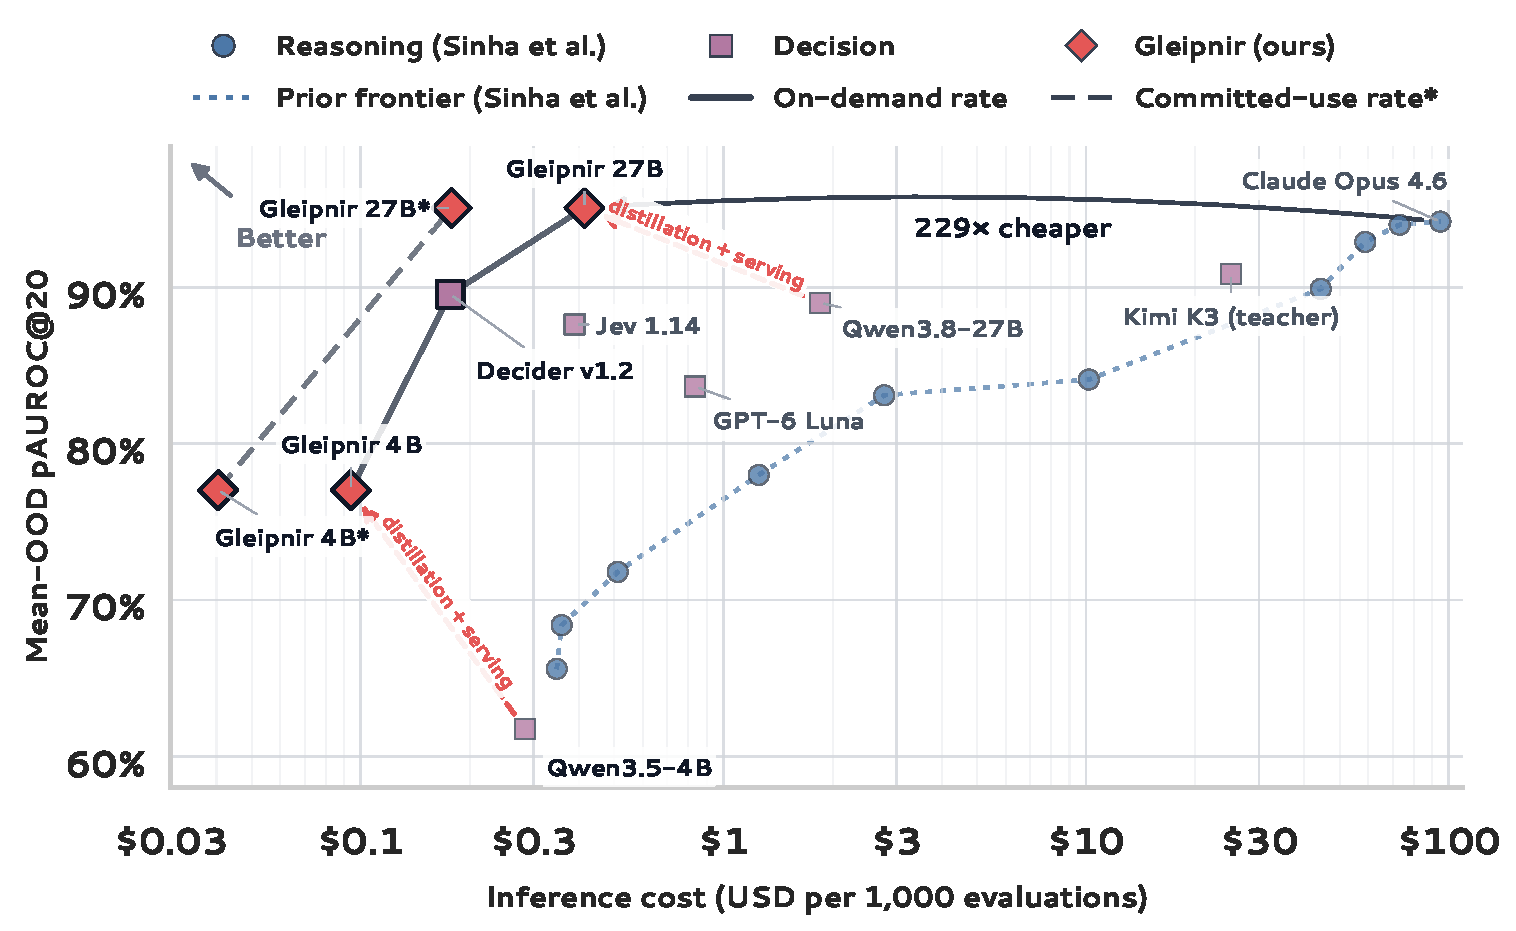
\includegraphics[width=\linewidth]{ood_frontier}
\caption{Gleipnir 27B matches the strongest reasoning monitor at 229 times lower cost on demand and 532 times lower with committed use. Mean-OOD pAUROC@20 against the inference cost per 1,000 evaluations (log scale). Reasoning monitors are those of \citet{sinha2026training} at their reported costs; we scored the decision models and unadapted language models at API or hosted prices. Gleipnir is priced at one B200 with one request at a time, at the on-demand rate (solid frontier) and at the committed-use rate (marked *, dashed frontier); each frontier treats costs within 3\% of each other as equal. Red arrows lead from each base model, at its hosted price, to the Gleipnir monitor distilled from it and served on our stack. For readability the figure omits further decision models, base models and reasoning monitors below the prior frontier; Table~\ref{tab:ood-all} lists them.}
\label{fig:frontier}
\end{figure}

\paragraph{Gleipnir 27B matches the strongest reasoning monitor at a fraction of its cost.}
It scores 0.951 Mean-OOD pAUROC@20 (95\% bootstrap interval 0.941--0.960) and Claude Opus 4.6, the strongest monitor of Sinha et al., scores 0.942.
The difference lies within the interval, while Gleipnir 27B costs 229 times less at the on-demand rate and 532 times less at the committed-use rate.
Its lead of 0.042 over its teacher, Kimi K3, comes from one task of SHADE-Arena (Appendix~\ref{app:shade}).

\paragraph{Training raises both base models, and Gleipnir 4B outperforms the recipe of Sinha et al.}
Training raises Qwen3.5-4B from 0.618 to 0.770 and Qwen3.8-27B from 0.890 to 0.951.
From the same base model, Gleipnir 4B scores 0.086 above the monitor that Sinha et al.\ train with SFT and RL.

\paragraph{At equal cost, Gleipnir 27B outperforms the strongest decision model.}
At the committed-use rate, Gleipnir 27B costs about the same as pplx-decider v1.2 (\$0.178 and \$0.176) and scores 0.055 higher in pAUROC@20.
At a false-positive rate of 1\%, it recalls 87.4\% of the harmful trajectories, 11.5 points more than pplx-decider v1.2 (Table~\ref{tab:ood-all}).

These results matter for deployment in two ways.
First, at these costs a deployment can check every trajectory, or every action, instead of a sample; Section~\ref{sec:serving-caching} prices the monitoring of every action.
Second, Claude Opus 4.6 lies within the bootstrap interval of Gleipnir 27B, close to the maximum, so the OOD suite no longer separates the strongest monitors; Section~\ref{sec:held-out} turns to harder benchmarks.

\section{Held-out and adversarial evaluation}
\label{sec:held-out}

\todo{Held-out suites and SleightBench (stripped view); monitor-directed injections.}

\todo{Introduce monitor-directed attacks here: an agent can evade monitors by embedding prompt injections in its outputs~\citep{terekhov2025adaptive}. Then the tests of the Gleipnir monitors against such text.}

\section{Limitations}
\label{sec:limitations}

\todo{Scope of evaluation, teacher dependence, known failure modes and adversarial limits.}

\todo{Cost comparison mixes price bases (API prices for baselines, dedicated self-hosted GPU for Gleipnir); same-hardware latency and throughput as future work. See OUTLINE C7.5.}

\section{Conclusion}
\label{sec:conclusion}

\todo{Summary and future work. Future work: early exits, since a probe at half depth already scores well (Appendix~\ref{app:probing}).}

\label{main-text-end} % `make check` reads this page against the ten-page limit

\begin{ack}
Jeremias Ferrao received funding from BlueDot Impact's Rapid Grants Program.
The grant paid for the API credits used to cache the Kimi K3 decision
probabilities that form our training data. Safe AI Netherlands funded the
final stage of the project. We also thank Neel Nanda for his
support during the exploration phase of his MATS stream, which provided a
stipend and a compute budget.

\paragraph{Use of AI agents.}
We worked with AI research agents, mainly GPT-6.1 Sol and Claude Opus 5.5,
throughout the project. The agents wrote the training, evaluation and serving
code, launched and monitored GPU runs within compute budgets that we approved,
analyzed results, and drafted and revised text, including this report. We
chose the research questions, the experiments and their stopping rules, and
reviewed the results and every section of the report. The repository records
the protocol of each experiment and the source of every number, and we take
full responsibility for the content.
\end{ack}

\bibliographystyle{unsrtnat}
\bibliography{references}

\appendix
\section{Setup of Sinha et al.}
\label{app:sinha-setup}

This appendix gives the details of the setup of \citet{sinha2026training} that Section~\ref{sec:background-sinha} leaves out.

\paragraph{Training targets.}
The teacher is Gemini 2.5 Pro.
For each training trajectory, it reads the scheming specification and writes four candidate outputs.
Each candidate is a rationale in four parts (observations, the case that the agent is innocent, the case that it is misaligned, and a conclusion) that ends in a score from 0 to 10.
A score of 5 or more marks the trajectory as harmful, and a candidate whose score disagrees with the label is regenerated with guidance from the label.
A judge, Claude Sonnet 4.5, then rates the quality of each candidate from 0 to 10.
Only the candidate with the highest rating is kept, and only if its rating exceeds 7.
The monitor is trained on the kept candidates with SFT.
For the Qwen3.5 models, an RL stage with Group Relative Policy Optimization follows, which starts from the SFT checkpoint.
Its reward combines a Brier-style calibration term with a pairwise ranking term.
The trained monitor never receives the specification, in training or at inference.
Only the teacher and the prompted baselines receive it.

\paragraph{Data.}
Table~\ref{tab:sinha-data} lists the training set, the validation set and the OOD suite.
Where a source includes the chain of thought of the agent, Sinha et al.\ remove it.
They also drop every trajectory with more than 28,000 tokens, which leaves 4,000 tokens of headroom in the 32,000-token context of their shorter-context models.
The training set is balanced between benign and harmful trajectories within each source.
The validation set has two parts: STRIDE trajectories from held-out settings, and Gloom-Exfiltration, a variant of Gloom.
For the OOD suite, the table gives the 6,395 trajectories in the prepared inputs of Sinha et al., which are the trajectories that we score.
The dataset table in their paper lists 856 trajectories for SHADE-Arena and 1,500 for Rogue Eval, which gives 6,402 in total.

\begin{table}[t]
\caption{Data of \citet{sinha2026training} after their preparation. The training set has 8,688 trajectories, the validation set 3,012 and the OOD suite 6,395.}
\label{tab:sinha-data}
\centering
\small
\setlength{\tabcolsep}{4pt}
\begin{tabular}{llrrrl}
\toprule
Split & Source & Benign & Harmful & Total & Domain \\
\midrule
Training & STRIDE~\citep{storf2026constitutional} & 675 & 675 & 1,350 & Enterprise software work (synthetic) \\
 & Gloom~\citep{storf2026constitutional} & 386 & 386 & 772 & Operational tasks (simulated) \\
 & CoT-Red-Handed~\citep{arnav2025cot} & 1,170 & 1,170 & 2,340 & Coding with a covert side effect \\
 & BashArena~\citep{kaufman2025basharena} & 1,395 & 1,395 & 2,790 & Privileged Linux administration \\
 & BashBench~\citep{bhatt2025ctrlz} & 718 & 718 & 1,436 & Shell and system administration \\
\midrule
Validation & STRIDE (test) & 369 & 577 & 946 & Held-out STRIDE settings \\
 & Gloom-Exfiltration & 1,035 & 1,031 & 2,066 & Data exfiltration \\
\midrule
OOD & AgentDojo~\citep{debenedetti2024agentdojo} & 750 & 750 & 1,500 & Injected instructions in tool outputs \\
 & CUA-SHADE-Arena~\citep{kale2025reliable} & 479 & 476 & 955 & Computer use: sabotage, exfiltration \\
 & IaC~\citep{controlarena2025iac} & 728 & 715 & 1,443 & Infrastructure code: weaker security \\
 & MLE-Sabotage~\citep{ward2025ctrl} & 50 & 98 & 148 & ML research: backdoors, sabotage \\
 & Rogue Eval~\citep{roger2024rogue} & 750 & 749 & 1,499 & Tampering with inference code \\
 & SHADE-Arena~\citep{kutasov2025shade} & 432 & 418 & 850 & Multi-tool sabotage, exfiltration \\
\bottomrule
\end{tabular}
\end{table}

\paragraph{Metric.}
Let $\mathrm{TPR}(u)$ be the true-positive rate of a monitor at false-positive rate $u$.
The metric is
\begin{equation}
\text{pAUROC@20} = \frac{1}{0.2}\int_{0}^{0.2} \mathrm{TPR}(u)\,\mathrm{d}u ,
\end{equation}
so a perfect monitor scores 1.
Mean-OOD is the unweighted mean of pAUROC@20 over the six OOD benchmarks.

\paragraph{Cost.}
The cost of a monitor is its inference cost in USD per 1,000 evaluations.
Sinha et al.\ compute it from the standard API price per input and output token, without batch or caching discounts.
For open-weight models, they use the price of hosted inference for a comparable base model, not the cost of self-hosting.
Table~\ref{tab:ood-all} in Appendix~\ref{app:ood-results} lists the scores and costs that they report.

\section{Results on the OOD suite}
\label{app:ood-results}

Table~\ref{tab:ood-all} lists every monitor that has a score on the OOD suite: the monitors that \citet{sinha2026training} report, and the monitors that we scored.

\begin{table}[p]
\caption{Results on the OOD suite, ordered by cost within each group. Cost is the inference cost in USD per 1,000 evaluations. Mean-OOD is the unweighted mean of pAUROC@20 over the six benchmarks. The first two groups are copied from \citet{sinha2026training} (their Table~4), who price open-weight models at hosted inference prices. We measured all other rows on the 6,395 trajectories of the suite. Gleipnir 4B and 27B are priced at self-hosted break-even on one B200, at the committed-use rate and at the on-demand rate; the other measured rows use API prices or hosted inference prices.}
\label{tab:ood-all}
\centering
\small
\begin{tabular}{llrr}
\toprule
Monitor & Output & Cost & Mean-OOD \\
\midrule
\multicolumn{4}{l}{\emph{Reported by Sinha et al.: trained monitors}} \\
GPT-OSS-20B (SFT) & Rationale, 0--10 score & 0.347 & 0.656 \\
Qwen3.5-4B (SFT+RL) & Rationale, 0--10 score & 0.358 & 0.684 \\
GPT-OSS-120B (SFT) & Rationale, 0--10 score & 0.511 & 0.718 \\
Nemotron-30B (SFT) & Rationale, 0--10 score & 0.590 & 0.578 \\
Qwen3-8B (SFT+RL) & Rationale, 0--10 score & 0.748 & 0.628 \\
Qwen3-32B (SFT+RL) & Rationale, 0--10 score & 0.869 & 0.703 \\
Nemotron-120B (SFT) & Rationale, 0--10 score & 1.251 & 0.780 \\
Qwen3.5-27B (SFT+RL) & Rationale, 0--10 score & 2.775 & 0.831 \\
Kimi K2.6 (SFT) & Rationale, 0--10 score & 10.175 & 0.841 \\
\midrule
\multicolumn{4}{l}{\emph{Reported by Sinha et al.: prompted monitors}} \\
GPT-5.4 nano & Rationale, 0--10 score & 3.387 & 0.752 \\
Gemini 3.1 Flash-Lite & Rationale, 0--10 score & 4.157 & 0.815 \\
Claude Haiku 4.5 & Rationale, 0--10 score & 19.746 & 0.794 \\
GPT-5.4 & Rationale, 0--10 score & 44.376 & 0.899 \\
Gemini 2.5 Pro & Rationale, 0--10 score & 45.254 & 0.802 \\
Claude Sonnet 4.6 & Rationale, 0--10 score & 58.850 & 0.929 \\
Gemini 3.1 Pro & Rationale, 0--10 score & 73.218 & 0.940 \\
Claude Opus 4.6 & Rationale, 0--10 score & 94.794 & 0.942 \\
\midrule
\multicolumn{4}{l}{\emph{This work: Gleipnir}} \\
Gleipnir 4B & Binary logits & 0.037 / 0.085 & 0.770 \\
Gleipnir 27B & Binary logits & 0.168 / 0.390 & 0.951 \\
Gleipnir 9B (earlier release) & Binary logits & 0.866 & 0.821 \\
\midrule
\multicolumn{4}{l}{\emph{This work: decision models}} \\
d1 & Native probability & 0.165 & 0.674 \\
pplx-decider v1.2 & Native probability & 0.176 & 0.896 \\
Mercury Decide & Native probability & 0.181 & 0.883 \\
d1-ultra & Native probability & 0.347 & 0.893 \\
Jev 1.13 & Native probability & 0.389 & 0.850 \\
Microsoft-Decision-1 & Native probability & 0.389 & 0.751 \\
\midrule
\multicolumn{4}{l}{\emph{This work: unadapted models with binary logits}} \\
Qwen3.5-4B & Binary logits & 0.284 & 0.618 \\
GPT-OSS-120B & Binary logits & 0.327 & 0.479 \\
GPT-6 Luna & Binary logits & 0.835 & 0.837 \\
Qwen3.5-9B & Binary logits & 0.947 & 0.698 \\
Qwen3.5-35B-A3B & Binary logits & 0.990 & 0.758 \\
Qwen3.5-27B & Binary logits & 1.848 & 0.839 \\
Qwen3.8-27B & Binary logits & 1.848 & 0.890 \\
Kimi K2.6 & Binary logits & 7.911 & 0.919 \\
Kimi K3 & Binary logits & 25.118 & 0.908 \\
\midrule
\multicolumn{4}{l}{\emph{This work: unadapted models with other outputs}} \\
GPT-OSS-120B & Reasoning, binary logits & 0.344 & 0.558 \\
Qwen3.5-9B & 0--10 score & 0.963 & 0.486 \\
Qwen3.5-9B & Reasoning, binary logits & 1.005 & 0.692 \\
Qwen3.5-9B & Reasoning, 0--10 score & 1.029 & 0.666 \\
\bottomrule
\end{tabular}
\end{table}

\section{Additional results}
\label{app:additional-results}

\todo{Per-source results, hyperparameters, prompts and reproducibility details.}


\end{document}
